%%
%% Automatically generated file from DocOnce source
%% (https://github.com/hplgit/doconce/)
%%
%%
% #ifdef PTEX2TEX_EXPLANATION
%%
%% The file follows the ptex2tex extended LaTeX format, see
%% ptex2tex: http://code.google.com/p/ptex2tex/
%%
%% Run
%%      ptex2tex myfile
%% or
%%      doconce ptex2tex myfile
%%
%% to turn myfile.p.tex into an ordinary LaTeX file myfile.tex.
%% (The ptex2tex program: http://code.google.com/p/ptex2tex)
%% Many preprocess options can be added to ptex2tex or doconce ptex2tex
%%
%%      ptex2tex -DMINTED myfile
%%      doconce ptex2tex myfile envir=minted
%%
%% ptex2tex will typeset code environments according to a global or local
%% .ptex2tex.cfg configure file. doconce ptex2tex will typeset code
%% according to options on the command line (just type doconce ptex2tex to
%% see examples). If doconce ptex2tex has envir=minted, it enables the
%% minted style without needing -DMINTED.
% #endif

% #define PREAMBLE

% #ifdef PREAMBLE
%-------------------- begin preamble ----------------------

\documentclass[%
oneside,                 % oneside: electronic viewing, twoside: printing
final,                   % or draft (marks overfull hboxes, figures with paths)
10pt]{article}

\listfiles               % print all files needed to compile this document

\usepackage{relsize,makeidx,color,setspace,amsmath,amsfonts,amssymb}
\usepackage[table]{xcolor}
\usepackage{bm,microtype}

\usepackage[pdftex]{graphicx}

\usepackage[T1]{fontenc}
%\usepackage[latin1]{inputenc}
\usepackage{ucs}
\usepackage[utf8x]{inputenc}

\usepackage{lmodern}         % Latin Modern fonts derived from Computer Modern

% Hyperlinks in PDF:
\definecolor{linkcolor}{rgb}{0,0,0.4}
\usepackage{hyperref}
\hypersetup{
    breaklinks=true,
    colorlinks=true,
    linkcolor=linkcolor,
    urlcolor=linkcolor,
    citecolor=black,
    filecolor=black,
    %filecolor=blue,
    pdfmenubar=true,
    pdftoolbar=true,
    bookmarksdepth=3   % Uncomment (and tweak) for PDF bookmarks with more levels than the TOC
    }
%\hyperbaseurl{}   % hyperlinks are relative to this root

\setcounter{tocdepth}{2}  % number chapter, section, subsection

% Tricks for having figures close to where they are defined:
% 1. define less restrictive rules for where to put figures
\setcounter{topnumber}{2}
\setcounter{bottomnumber}{2}
\setcounter{totalnumber}{4}
\renewcommand{\topfraction}{0.95}
\renewcommand{\bottomfraction}{0.95}
\renewcommand{\textfraction}{0}
\renewcommand{\floatpagefraction}{0.75}
% floatpagefraction must always be less than topfraction!
% 2. ensure all figures are flushed before next section
\usepackage[section]{placeins}
% 3. enable begin{figure}[H] (often leads to ugly pagebreaks)
%\usepackage{float}\restylefloat{figure}

% newcommands for typesetting inline (doconce) comments
\newcommand{\shortinlinecomment}[3]{{\color{red}{\bf #1}: #2}}
\newcommand{\longinlinecomment}[3]{{\color{red}{\bf #1}: #2}}

% prevent orhpans and widows
\clubpenalty = 10000
\widowpenalty = 10000

% --- end of standard preamble for documents ---


% insert custom LaTeX commands...

\raggedbottom
\makeindex

%-------------------- end preamble ----------------------

\begin{document}

% endif for #ifdef PREAMBLE
% #endif


% ------------------- main content ----------------------



% ----------------- title -------------------------

\thispagestyle{empty}

\begin{center}
{\LARGE\bf
\begin{spacing}{1.25}
FFM232, Klassisk fysik och vektorfält - Föreläsningsanteckningar
\end{spacing}
}
\end{center}

% ----------------- author(s) -------------------------

\begin{center}
{\bf \href{{http://fy.chalmers.se/subatom/tsp/}}{Christian Forssén}, Institutionen för fysik, Chalmers, Göteborg, Sverige${}^{}$} \\ [0mm]
\end{center}

\begin{center}
% List of all institutions:
\end{center}
    
% ----------------- end author(s) -------------------------

% --- begin date ---
\begin{center}
Sep 22, 2016
\end{center}
% --- end date ---

\vspace{1cm}


\subsection{Repetition: Integralsatser}

\begin{itemize}
\item Gauss sats
\end{itemize}

\noindent
\begin{equation}
  \int_V \nabla \cdot \vec{F} \mbox{d}V = \oint_{\partial V} \vec{F} \cdot \mbox{d} \vec{S}.
\end{equation}
\begin{itemize}
\item Stokes sats
\end{itemize}

\noindent
\begin{equation}
  \int_S \left( \nabla \times \vec{F}\right) \cdot \mbox{d}\vec{S} = \oint_{\partial S} \vec{F}\cdot
\mbox{d}\vec{r},
\end{equation}
Gäller för kontinuerligt deriverbara vektorfält. Vad händer om fältet har en singularitet?

\section{6. Singulära fält}

Det finns tre viktiga typer av singulariteter, vilka dyker upp för speciella vektorfält:

\begin{itemize}
\item Punktkälla 

\item Linjeälla 

\item Virveltråd
\end{itemize}

\noindent
\subsection{Punktkällor}

Ett fält av formen 
\begin{equation}
  \vec{F} = \frac{q}{4 \pi r^2}\hat{e}_{r}
\end{equation}
kallas för fältet från en punktkälla med styrkan $q$. Med lämplig tolkning av konstanten $q$ kan detta t.ex. föreställa det elektriska fältet från en laddning i origo, eller gravitationsfältet från en massa i origo.  

\shortinlinecomment{Comment 1}{ Notera att detta fält är singulärt i origo. Skissa gärna fältlinjerna. }{ Notera att detta fält }

Detta fält är rotationsfritt (åtminstone för $r>0$)
\begin{equation}
\nabla\times\vec F = \frac{1}{r^2\sin\theta}
\begin{vmatrix}
\hat{e}_r&r\hat{e}_\theta&r\sin\theta\hat{e}_\varphi \\ 


\frac{\partial}{\partial r}&
\frac{\partial}{\partial \theta}&
\frac{\partial}{\partial \varphi} \\ 
F_r(r)&0&0
\end{vmatrix}=0
\end{equation}
Rotationsfriheten är också en direkt följd av att $\vec F = - \nabla \phi$ med den skalära potentialen 
\begin{equation}
\phi=\frac{q}{4\pi r}
\end{equation}

Vektorfältet $\vec F$ är också divergensfritt (för $r>0$)
\begin{equation}
\nabla\cdot\vec F=\frac{1}{r^2}
 \frac{\partial}{\partial r}\left(r^2 \frac{q}{4\pi
r^2}\right)=0, \quad r>0
\end{equation}

\longinlinecomment{Comment 2}{ Trots frånvaron av divergens får vi ett resultat skilt från noll om vi beräknar normalytintegralen av $\vec F$ över en yta som omsluter origo. Detta görs enklast genom att utföra integralen över en sfär med radien $a$. }{ Trots frånvaron av divergens }

Normalytintegralen för en yta (sfäriskt skal, radie $a$) som omsluter origo:
\begin{equation}
\label{eq:punktkalla}
\int_S\vec F\cdot d\vec S= 
\frac{q}{4\pi a^2} 4\pi a^2=q
\end{equation}
medan Gauss sats skulle ge $\int_V \nabla \cdot \vec{F} \mbox{d}V = 0 $!

\longinlinecomment{Comment 3}{ En viktig slutsats är att det vore fel att naivt tillämpa Gauss sats på en volym innehållande origo, trots att fältet ser divergensfritt ut. Det beror på att det är singulärt där. Med vår nuvarande kunskap får vi acceptera att vi måste undvika punkter där fält är singulära när vi använder integralsatser. }{ En viktig slutsats är }

Mer allmänt:
\begin{equation}
\oint_S \vec F\cdot d\vec S= 
\left\{
\begin{array}{ll}
0 & \mathrm{om~ytan~inte~omsluter~origo.} \\ 
q & \mathrm{om~ytan~omsluter~origo.}
\end{array}
\right.
\end{equation}

Anledningen till att vi inte kan använda Gauss sats är
\begin{equation}
\nabla \cdot \vec{F} = 
\left\{
\begin{array}{ll}
0 & r \neq 0 \\ 
\infty & r=0 \mathrm{~(bättre~definition~kommer~senare)}
\end{array}
\right.
\end{equation}

\paragraph{Flöde från punktkälla genom allmän yta.}
En mer förfinad version av ekv. (\ref{eq:punktkalla}) för normalytintegralen av fältet från en punktkälla över en godtycklig yta $S$ kan fås genom att dela upp normalytelementet i $r$-, $\theta$- och $\varphi$-ytor. Den relevanta projektionen är den på $r$-ytan eftersom fältet har den riktningen
\begin{equation}
\mbox{d}\vec{S}_r = \pm \hat{e}_r h_\theta h_\varphi \mbox{d}\theta \mbox{d}\varphi 
\end{equation}
där tecknet beror på om normalen för $S$ är utåtriktad (positiv) eller inåtriktad (negativ). Detta ger 
\begin{equation}
\frac{q}{4\pi} \int_S \frac{\hat{e}_r\cdot d\vec S}{r^2} = \pm \frac{q}{4\pi} \iint \sin\theta \mbox{d}\theta \mbox{d}\varphi = q \frac{\Omega}{4\pi} 
\end{equation}
där $\Omega$ är den rymdvinkel ytan $S$ tar upp sedd från origo. Läs mer om begreppet rymdvinkel: \href{{http://mathworld.wolfram.com/SolidAngle.html}}{\nolinkurl{http://mathworld.wolfram.com/SolidAngle.html}}

T.ex. blir rymdvinkeln för en yta som omsluter origo
\begin{equation}
\int_{\theta=0}^\pi \int_{\varphi=0}^{2\pi} \sin\theta \mbox{d}\theta \mbox{d}\varphi = 4\pi.
\end{equation}

\subsection{Linjekällor}

Ett fält av typen
\begin{equation}
  \vec{F} = \frac{k}{2 \pi \rho} \hat{e}_{\rho}
\end{equation}
svarar fysikaliskt till exempel emot en laddning som är jämnt fördelad längs med en linje (i det här fallet $z$-axeln). Storheten $k$ motsvarar då laddning/längdenhet. Linjekällan är då källan till ett fält som överallt pekar radiellt ut från $z$-axeln 

\shortinlinecomment{Rita 4}{ Fält för linjekälla genom $z$-axeln. }{ Fält för linjekälla genom }.

Fältet är divergensfritt $\nabla \cdot \vec{F} = 0$, förutom för $\varrho=0$.

Det kan erhållas från potentialen 
\begin{equation}
	\phi=-\frac{k}{2\pi}\log\frac{\varrho}{\varrho_0}
\end{equation}
Med konstant källtäthet fås normalytintegralen för en cylinder med längden $L$ som omsluter linjekällan längs $z$-axeln
\begin{equation}
	\int_S \vec{F} \cdot \mbox{d}\vec{S} = k L
\end{equation}

\longinlinecomment{Comment 5}{ Mer generellt blir normalytintegralen av fältstyrkan över en smal tub nära en godtycklig kurva lika med den inneslutna källan $q(C)=\int_C k(\vec{r}) ds$, där $C$ är den del av kurvan som innesluts av tuben. }{ Mer generellt blir normalytintegralen }

\subsection{Ytkälla}

På motsvarande sätt kan vi tala om ytkällor i tre dimensioner. Fältet 
\begin{equation} 
\vec F=\frac{\sigma}{2}\mathrm{sign}(z)\hat{z}
\end{equation}
motsvar en ytkälla i $xy$-planet (vid $z=0$), där $\sigma$, i det elektrostatiska fallet, skulle kallas för en ytladdningstäthet.

Närvaron av en ytkälla på ytan $S$ med styrkan $\sigma$ är liktydigt med att
normalkomponenten av $\vec F$ har en diskontinuitet enligt $\hat n\cdot(\vec F_+-\vec F_-)=\sigma$, där $\vec F_+$ är fältets värde på den sida dit normalen pekar, och $\vec F_-$ dess värde på motsatta sidan.


\paragraph{Källtäthet.}


\vspace{3mm}


Vi har nu sett hur olika singulariteter kan vara källor till ett fält $\vec{F}$.  Analogt med detta kan vi tolka $\nabla \cdot \vec{F}$ som en utbredd källa till $\vec{F}$.  Därför kallar man ibland $\nabla \cdot \vec{F} = \rho$ för källtäthet.

\begin{itemize}
\item Singulära källor: $\nabla \cdot \vec{F} = 0$ utom på vissa ställen 
\end{itemize}

\noindent
\subsection{Virveltråd}

Fältlinjerna till det singulära fältet
\begin{equation}
  \vec{F} = \frac{J}{2 \pi \rho} \hat{e}_{\varphi}
\end{equation}
bildar koncentriska cirklar kring $z$-axeln.  Därför säger vi att det finns en virveltråd med styrkan $J$ på $z$-axeln.  

Divergensfritt: $\nabla \cdot \vec{F} = 0$.

Rotationen av fältet:
\begin{equation}
\nabla\times\vec F=\frac{1}{\varrho}
	\begin{vmatrix}
        \hat{e}_\varrho&\varrho\hat{e}_\varphi&\hat z \\ 
        \frac{\partial}{\partial \varrho} & 
\frac{\partial}{\partial \varphi}
        & 
\frac{\partial}{\partial z} \\ 
        0 & \varrho \frac{J}{2\pi\varrho} & 0
    \end{vmatrix} = 0, \quad \mathrm{för~} \varrho > 0.
\end{equation}

Stokes sats skulle ge
\begin{equation}
	\oint_{\partial S} \vec{F} \cdot \mbox{d} \vec{r} = \int_S \left( \nabla \times \vec{F} \right) \cdot \mbox{d} \vec{S} = 0,
\end{equation}
men vad skulle ske om ytan $S$ gick genom singulariteten?

\shortinlinecomment{Rita 6}{ en cirkel med radien $a$ runt $z$-axeln, $\mbox{d}\vec{r} = a \hat{e}_\varphi \mbox{d} \varphi$ }{ en cirkel med radien }

Linjeintegralen blir
\begin{equation}
\int_C\vec F\cdot \mbox{d}\vec r = \int_{\varphi=0}^{2\pi} \frac{J}{2 \pi a} a \mbox{d} \varphi = J.
\end{equation}
Generellt gäller detta resultat för en kurva $C$ som omsluter $z$-axeln ett varv i positiv led, medan integralen blir noll för kurvor som inte omsluter $z$-axeln. 

Det vanligaste exemplet är det statiska magnetiska fältet från en ström. Dvs fältet är $\vec{B}$ och $J$ motsvarar den elektriska strömmen.

\paragraph{Virveltäthet.}
Vi har nu sett hur en virveltråd kan alstra en virvel i ett vektorfält. Det kan också uppstå virvlar i fält som saknar singulariteter, och för att få ett mått på omfattningen av sådana virvlar inför man virveltätheten $\nabla \times \vec{F}$.

\begin{itemize}
\item Singulära virvlar: $\nabla \times \vec{F} = 0$ utom på vissa ställen 
\end{itemize}

\noindent
---------------------------------------------

\paragraph{Exempel: 6.3.}
Beräkna integralen $\oint_C \vec F \cdot d\vec{r}$, $C$: $x^2 + \frac{y^2}{4} = a^2$ och $z = 0$ (som genomlöps i positiv riktning) och 
\begin{equation}
  \vec F = F_0 \left[\frac{\varrho \sin 2\varphi}{2a} \hat{e}_\varrho
+ \left(\frac{a}{\varrho} - \frac{\varrho \sin^2 \varphi}{a}\right)\hat{e}_\varphi
\right]
\end{equation}
$F_0$ och $a$ är konstanter.

\emph{Lösning}:  

\longinlinecomment{Comment 7}{ Kurvan $C$ är en ellips med centrum i origo och halvaxlarna $a$ och $2a$. Enligt högerhandsregeln väljer vi $\hat z$ som normal till ellipsskivan. }{ Kurvan $C$ är en }

$C$ kan parametriseras $(x,y) = (a\cos\varphi,2a\sin\varphi)$.

Dela upp $\vec{F} = \vec{F}_1 + \vec{F}_2$ där $\vec F_1=F_0 \frac{a}{\varrho}\hat{e}_\varphi$ innehåller fältets singularitet
(motsvarar en virveltråd på $z$-axeln med styrkan $2\pi F_0a$). 

Kurvan $C$ omsluter virveltråden en gång i positiv led så att $\oint_C \vec{F}_1 \cdot d\vec{r} = 1 \cdot 2\pi F_0a$

Bidraget från $\vec F_2$ fås enklast med hjälp av Stokes sats. Rotationen blir
\begin{equation}
  \nabla \times\vec{F}_2 = \frac{F_0}{\rho} 
  	\begin{vmatrix}
	\hat{e}_\varrho & \varrho \hat{e}_\varphi & \hat z \\ 
	\frac{\partial}{\partial \varrho} & \frac{\partial}{\partial \varphi} &
                       \frac{\partial}{\partial z} \\ 
	\frac{\varrho \sin 2\varphi}{2a} & -\frac{\varrho^2\sin^2 \varphi}{a} & 0
	\end{vmatrix} =- \frac{F_0}{a}\hat z
\end{equation}

Detta ger 
\begin{equation}
\oint_C \vec{F}_2 \cdot \mbox{d}\vec{r} = \int_S \left( - \frac{F_0}{a}\hat z \right) \cdot \hat{z} \mbox{d}S = - \frac{F_0}{a} \pi \cdot a \cdot 2a = - 2 \pi F_0 a
\end{equation}
Värdet på den totala integralen blir alltså $\oint_C (\vec{F}_1 + \vec{F}_2) \cdot \mbox{d}\vec{r} = 0$.

\subsection{Superposition: beräkning av fält från allmänna källfördelningar}

\paragraph{Punktkälla i origo.}
Fältet i punkten $\vec{r}$
\begin{equation}
  \vec{F}(\vec{r}) = \frac{q}{4 \pi r^2} \hat{e}_r,
\end{equation}
vilket fås av potentialen
\begin{equation}
  \phi(\vec{r}) = \frac{q}{4 \pi r},
\end{equation}
eftersom
\begin{equation}
  \vec{F}(\vec{r}) = -\nabla \phi(\vec{r}) = - \hat{e}_r \partial_r \frac{q}{4 \pi r} = \frac{q}{4 \pi r^2} \hat{e}_r.
\end{equation}

\paragraph{Punktkälla i punkten $\vec{r}\,'$.}
Potentialen i punkten $\vec{r}$ blir uppenbart lika med
\begin{equation}
  \phi(\vec{r}) = \frac{q}{4 \pi \left| \vec{r} - \vec{r}\,' \right|}.
\end{equation}
Detta ger fältet
\begin{align}
  \vec{F}(\vec{r}) &= -\nabla \phi(\vec{r}) = - \left( \hat{x}\partial_x + \hat{y}\partial_y + \hat{z}\partial_z \right) \frac{q}{4 \pi \sqrt{(x-x')^2 + (y-y')^2 + (z-z')^2}} \nonumber \\ 
  &= - \frac{q}{4 \pi} \left( -\frac{1}{2} \right) \frac{ 2(x-x')\hat{x} + 2(y-y')\hat{y} + 2(z-z')\hat{z}}{ \left[ (x-x')^2 + (y-y')^2 + (z-z')^2 \right]^{3/2}} \nonumber \\ 
  &= \frac{q (\vec{r} - \vec{r}\,' )}{4 \pi \left| \vec{r} - \vec{r}\,' \right|^3}.
\end{align}

\paragraph{Allmän linjekälla.}
Betrakta en linjekälla längs kurvan $C$ som ges av $\vec{r} = \vec{r}(\tau)$. Linjekällan har linjekälltätheten $k(\tau)$, som alltså inte nödvändigtvis är konstant.

VI kan dela upp linjen i infinitesimala linjeelement $\mbox{d}s$, vardera med laddningen $\mbox{d}q = k\left(\vec{r}(\tau)\right) \mbox{d}s$ (som alltså blir en funktion av $\tau$). Vi kan betrakta dessa linjelement som punktkällor. Bidraget från en sådan källa till potentialen i en (godtycklig) punkt $\vec{r}$ är
\begin{equation}
\mbox{d}\phi(\vec{r}) = \frac{k\left(\vec{r}\,'(\tau)\right) \mbox{d}s'}{4 \pi \left| \vec{r} - \vec{r}\,' \right|}
\end{equation}
Genom att summera alla dessa bidrag, dvs integrera längs linjen $C$, får vi den totala potentialen i punkten $\vec{r}$
\begin{equation}
\phi(\vec{r}) = \int_C \frac{k\left(\vec{r}\,'\right) \mbox{d}s'}{4 \pi \left| \vec{r} - \vec{r}\,' \right|}.
\end{equation}
Notera att $\vec{r}\,' = \vec{r}\,'(\tau)$ och att $\mbox{d}s' = \left| \frac{\mbox{d}\vec{r}\,'}{\mbox{d}\tau} \right| \mbox{d}\tau$

\paragraph{Allmän ytkälla.}
Betrakta en ytkälla längs kurvan $S$ som ges av $\vec{r} = \vec{r}(s,t)$. Ytkällan har ytkälltätheten $\sigma\left( \vec{r}(s,t) \right)$.

Genom att summera alla bidrag från infinitesimala ytelement får vi den totala potentialen i punkten $\vec{r}$
\begin{equation}
\phi(\vec{r}) = \int_S \frac{\sigma\left(\vec{r}\,'\right) \mbox{d}S'}{4 \pi \left| \vec{r} - \vec{r}\,' \right|}.
\end{equation}

\paragraph{Allmän rymdkälla.}
En allmän rymdkälla har en rymdkälltätheten som ges av $\rho\left( \vec{r} \right) = \nabla \cdot \vec{F} \left( \vec{r} \right)$. Återigen kan vi använda superposition för att få den totala potentialen i punkten $\vec{r}$
\begin{equation}
\phi(\vec{r}) = \int_V \frac{\rho\left(\vec{r}\,'\right) \mbox{d}V'}{4 \pi \left| \vec{r} - \vec{r}\,' \right|}.
\end{equation}

\paragraph{Exempel: 6.4.}
Vad är potentialen från en ytkälla med konstant täthet $\sigma_0$, belägen på cirkelskivan med radie $a$ i $(x,y)$-planet med $z$-axeln som symmetriaxel? Speciellt, vad är
potentialen på $z$-axeln?

\emph{Lösning}:
Beteckna ortvektorn för en punkt på källan med $\vec{r}\,'$  och ortvektorn för punkten vi vill veta potentialen i med $\vec{r}$. 

Problemets symmetri gör det lämpligt att använda cylindriska koordinater. Vi får lägesvektorn $\vec{r} = \rho \hat{\rho} + z \hat{z}$ för punkten. Punkter på källan kan beskrivas med lägesvektorn $\vec{r}\,' = \rho' \hat{\rho}$ (notera att $z'=0$ eftersom ytkällan ligger i $xy$-planet).



% inline figure
\centerline{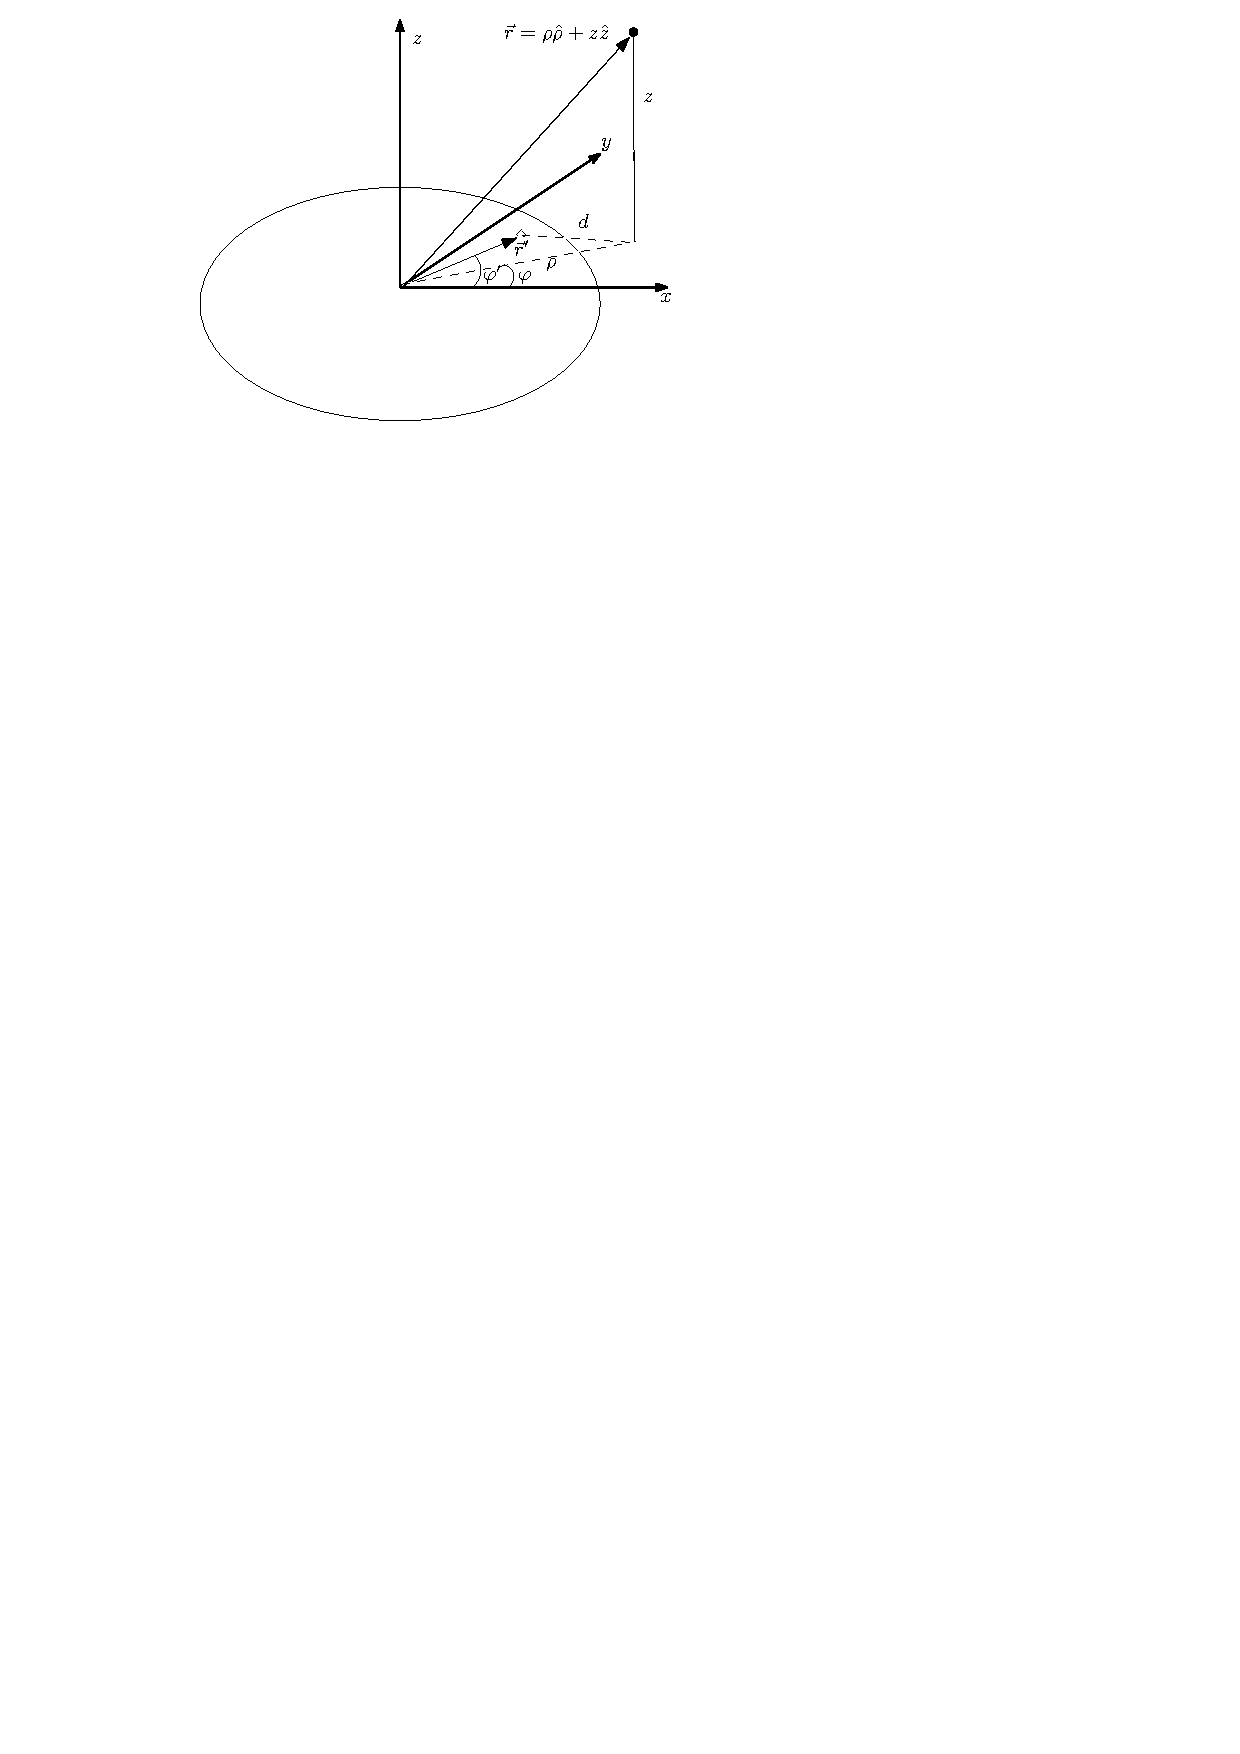
\includegraphics[width=0.8\linewidth]{fig/ex6_4.pdf}}



Vi får avståndet mellan de två punkterna som
\begin{equation}
|\vec{r}-\vec{r}\,'|
= \sqrt{d^2 + z^2}
=\sqrt{\varrho^2+\varrho'^2-2\varrho\varrho'\cos(\varphi-\varphi')+z^2}
\end{equation}
med hjälp av cosinusteoremet.
Med superposition kan vi teckna ett explicit uttryck för potentialen:
\begin{equation}
\phi(\vec{r})=\int_0^a d\varrho'\int_0^{2\pi}d\varphi'\,
\varrho'\frac{\sigma_0}{4\pi \sqrt{\varrho^2+\varrho'^2-2\varrho\varrho'\cos(\varphi-\varphi')+z^2}}
\end{equation}

Om $\vec{r}$ ligger på $z$-axeln förenklas uttrycket till
\begin{align}
\phi(0,0,z) &= \int_0^a d\varrho'\int_0^{2\pi}\mbox{d}\varphi'\,
\varrho'\frac{\sigma_0}{4\pi \sqrt{\varrho'^2+z^2}}
=\frac{\sigma_0}{2}\left[\sqrt{\varrho'^2+z^2}\right]_{\varrho'=0}^a \\ 
&=\frac{\sigma_0}{2}\left(\sqrt{z^2+a^2}-|z|\right).
\end{align}
Vi kan kontrollera vad som händer då $|z|\rightarrow+\infty$. Då är 
\begin{equation}
\sqrt{z^2+a^2}-|z|=|z|(\sqrt{1+a^2/z^2}-1) = |z|
\left( 1+\frac{a^2}{2z^2}+\mathcal{O}(\frac{a^3}{z^3})-1\right) \approx \frac{a^2}{2|z|},
\end{equation}
så $\phi(0,0,z)\approx \frac{a^2\sigma_0}{4|z|}$, vilket är fältet från en punktkälla med styrka $\pi a^2\sigma_0$. Befinner vi oss långt bort från ytkällan (dvs $z \gg a$) så ser fältet ut som fältet från en punktkälla. Det verkar rimligt!

\subsection{Greensfunktion}

Funktionen
\begin{equation}
G\left( \vec{r},\vec{r}\,' \right) = \frac{1}{4 \pi \left| \vec{r} - \vec{r}\,' \right|},
\end{equation}
kallas \emph{Greensfunktionen} och kan sägas motsvara bidraget till potentialen i punkten $\vec{r}$ från en punktkälla med styrkan 1 belägen i punkten $\vec{r}\,'$. Dessa funktioner dyker upp igen i kapitel 9. Vi kan alltså skriva fältet från en allmän rymdkälla
\begin{equation}
\phi(\vec{r}) = \int_V \rho\left(\vec{r}\,'\right) G\left( \vec{r},\vec{r}\,' \right) \mbox{d}V'.
\end{equation}

\subsection{Multipoler}

Fältet
\begin{equation}
  \vec{F} = \frac{q}{4 \pi r^2} \hat{e}_{r}
\end{equation}
kallas för ett monopolfält.  Det kan finnas fält vars styrka avtar snabbare med $r$, men sådana fält innehåller praktiskt taget alltid ett vinkelberoende. Ett exempel på ett sådant fält är dipolfältet, dvs.~två lika och motsatta laddningar nära varandra. 

Lägg en laddning $q = \frac{\mu}{\varepsilon}$ på $(x,y,z)=(0,0,\varepsilon)$ och en laddning
$-q = -\frac{\mu}{\varepsilon}$ i origo. Potentialen från de båda laddningarna tillsammans blir
\begin{equation}
\phi(\vec{r})=\frac{\mu/\varepsilon}{4\pi|\vec{r}-\varepsilon\hat z|}-\frac{\mu/\varepsilon}{4\pi r}
\end{equation}
Vi kan skriva $|\vec{r}-\varepsilon \hat z|=\sqrt{\varrho^2+(z-\varepsilon)^2}$, och om
$\varepsilon$ är litet ($\varepsilon/\varrho,\varepsilon/z \ll 1$) blir detta $\sqrt{\varrho^2+z^2-2\varepsilon
z}=\sqrt{r^2-2\varepsilon z}\approx r(1-\frac{\varepsilon z}{r^2})$. Så $\frac{1}{|\vec{r}-\varepsilon\hat z|}\approx \frac{1}{r}(1+\frac{\varepsilon z}{r^2})$.

\longinlinecomment{Comment 8}{ Här har vi använt Taylorutvecklingarna $\sqrt{1-x} = 1 - \frac{x}{2} + \mathcal{O}(x^2)$ samt $\frac{1}{1-x} = 1 + x + \mathcal{O}(x^2)$. }{ Här har vi använt }

Potentialen blir
\begin{equation}
\phi(\vec{r})\approx\frac{\mu}{4\pi\varepsilon}\left[\frac{1}{r}\left(1+\frac{\varepsilon z}{r^2}\right)-\frac{1}{r}\right]=\frac{\mu z}{4\pi r^3}=\frac{\mu\cos\theta}{4 \pi r^2}
\end{equation}
Mer generellt kan man skriva $\phi=\frac{\vec\mu\cdot\vec{r}}{4 \pi r^3}$. I vårt fall var alltså $\vec\mu=\mu\hat z$ dipolmomentet (som alltså ges av produkten av laddningen $\frac{\mu}{\varepsilon}$ och separationsvektorn $\varepsilon\hat z$).

Fältet blir
\begin{equation}
  \vec{F} = \frac{\mu}{4 \pi r^3} \left(\cos \theta \hat{e}_{r} + \sin \theta
\hat{e}_{\theta}\right).
\end{equation}
Notera att fältlinjerna är vinkelräta mot nivåkurvorna (eftersom $\vec{F} = -\nabla \phi$). I detta fall kommer de alltså att vara cirklar med centrum längs $x$-axeln.

Om man integrerar dipolfältet över en sfär ser man att integralen blir 0.  Detta beror på att man kan se fältet som sammansatt av en positiv och en negativ laddning på ett litet avstånd från varandra. Det går också att definiera kvadrupolfält, oktopolfält och så vidare.




% inline figure
\centerline{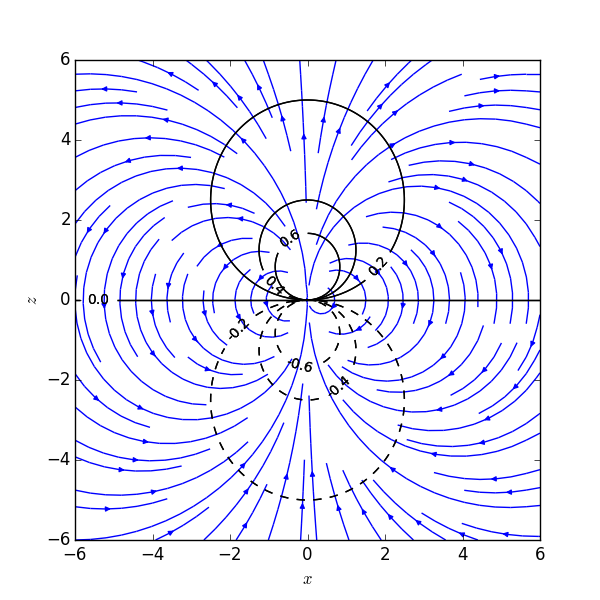
\includegraphics[width=0.8\linewidth]{fig/dipole_fieldplot.png}}



% ------------------- end of main content ---------------


% #ifdef PREAMBLE
\printindex

\end{document}
% #endif

